\documentclass{article}
\usepackage[utf8]{inputenc}
\usepackage{geometry}
\usepackage[dvipsnames]{xcolor}
\usepackage{graphicx}
\usepackage{hyperref}
\usepackage[english]{babel}

\setlength{\parindent}{1em}
\setlength{\parskip}{1em}
\geometry{margin=1.5cm}

\title{\Huge{\textbf{How to use the Template}} \\ \normalsize{Made to help you organize and easily make your page}}
\author{\normalsize{By} \\ \large{CSS Leaders: Marco Biasion and Bojan Lazarevski}}
\date{}


\begin{document}

\maketitle

\section*{Follow the Steps:}
\begin{itemize}
    \item Update the working repository by issuing the following command on your terminal:
    \colorbox{grey!7}{\texttt{svn update}} \\
    \textit{Note: make sure you update the repository every time before you start working on your files!}
    
    \item Access the folder with path \colorbox{grey!7}{\texttt{web/html/}}. Here, you will find a folder named \colorbox{grey!7}{\texttt{TEMPLATE}}. Copy and paste it in the same location \colorbox{grey!7}{\texttt{(web/html/)}}. Then, rename the folder you have just pasted by following this format: \colorbox{grey!7}{\texttt{generation-name\_product-name}}, all in lowercase. \\
    \textit{Example:} \texttt{gen0\_pong}
    
    \item Inside this folder, you will find a file named \colorbox{grey!7}{\texttt{TEMPLATE.html}}. Rename it by just inserting the name of your product. \\
    \textit{Example: } \texttt{super\_mario\_64}. \\
    \textit{Note: Use underscores (} \texttt{\_} \textit{) instead of spaces.} \\
    \textit{Note: Do not insert the generation in the name of the file:} \texttt{gen\_0\_super\_mario\_64} \textit{or} \texttt{super\_mario\_64\_generation\_0}
    
    \item Open the file with your preferred text editor.
    
    \item Now you have to set the meta tags containing the information about your page:
    \begin{figure}[h]
        \centering
        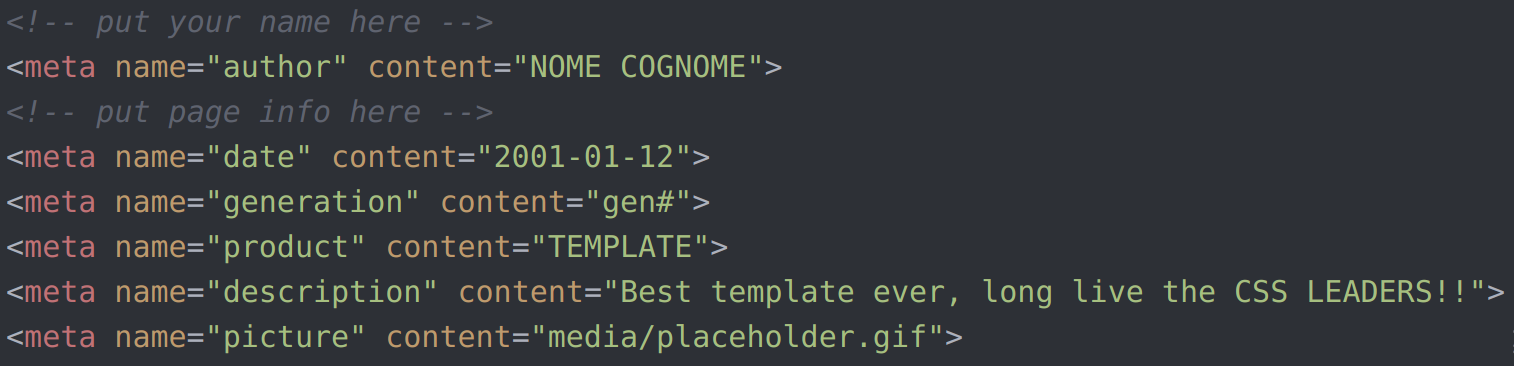
\includegraphics[height=3.6cm]{meta_tags.png}
    \end{figure}
    \begin{itemize}
        \item \texttt{author} is your name and surname, capitalized.\\
        \textit{Example:} \texttt{content="Bojan Biasion"}
        \item \texttt{date} is the date the product was launched, year-month-day.\\
        \textit{Example:} \texttt{content="2001-12-01"}
        \item \texttt{generation} is the generation of the product.\\
        \textit{Example:} \texttt{content="gen0"}
        \item \texttt{product} is the name of the product.\\
        \textit{Example:} \texttt{content="pong"} \textit{or} \texttt{Super Mario 64}
        \item \texttt{description} is a short description of your product.\\
        \textit{Example:} \texttt{content="Best product ever!!"}
        \item \texttt{picture} is the placeholder of the product in the timeline, it has to be a square and it should be an animated gif.\\
        \textit{Note: it's not necessary that it's an animated gif, but it's highly appreciated.}
    \end{itemize}
    
    \item Below the meta tags, you will find links to the stylesheets. Change the stylesheet \colorbox{grey!7}{\texttt{generation-style}} with the proper generation style URL. \\
    \textit{Example:} \texttt{href="styles/gen0/style.css"}
    \begin{figure}[h]
        \centering
        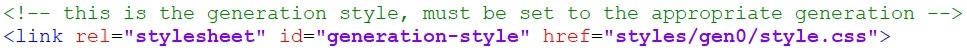
\includegraphics[height=0.8cm]{generation.jpg}
    \end{figure}
    
    \item After that you will find the stylesheet \colorbox{grey!7}{\texttt{user-style}} here you are can use the variables to personalize the page. \\
    \textit{Note: all the path must be relative to the page.}
    \begin{itemize}
        \item[] \texttt{--background-image-left: url( "media/FILE" );} \textit{The left background image}
        \item[] \texttt{--background-image-right: url( "media/FILE" );} \textit{The right background image}
        \item[] \texttt{--background-fade-color: COLOR;} \textit{The fading color between the background images}
        \item[] \texttt{--banner-image: url( "media/FILE" );} \textit{The image containing the logo of the product}
        \item[] \texttt{--banner-color: COLOR;} \textit{The color behind the logo, useful only if the image has transparency}
        \item[] \texttt{--audio-file: url( "media/FILE" );} \textit{The audio file to play on the page}
        \item[] \texttt{--container-background-color: COLOR;} \textit{The color of the container which contains the page content}
        \item[] \texttt{--container-text-color: COLOR;} \textit{The color of the text in the container}
        \item[] \texttt{--container-border-color: COLOR;} \textit{The color of the border of the container}
        \item[] \texttt{--index-background-color: COLOR;} \textit{The background color of the index of the page}
        \item[] \texttt{--index-text-color: COLOR;} \textit{The color of the text in the index of the page}
        \item[] \texttt{--index-border-color: COLOR;} \textit{The color of the border of the index of the page}
        \item[] \texttt{--link-color-hover: COLOR;} \textit{The color of the links ('a' element) when you hover over them}
        \item[] \texttt{--scrollbar-thumb: COLOR;} \textit{The color of the scroll bar in the container}
    \end{itemize}
    You are also allowed to add your own personalized CSS code. \\
    \textbf{Remark 1:} All web pages in a certain generation should look somewhat similar. Therefore, do not change everything that you can. Make sure the changes you apply do not deviate too much the style of the page from the generation one.\\
    \textit{Note: When you change something, share the information with your group, if many of you applied the same change(s), contact the CSS Leaders to see if it can be included directly in the} \texttt{generation-style}. \\
    
    \item You can now start inserting the content in the page. Make sure to put everything in the content div (\colorbox{grey!7}{\texttt{<div id="content">}}). Each section and subsection of your page (h2, h3) must have an unique id. \\
    \textit{Example: } \texttt{<h2 id="s1">The beginning of the project</h2>}
    \begin{figure}[h]
        \centering
        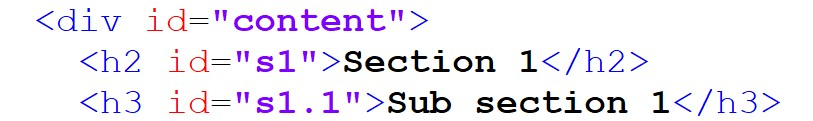
\includegraphics[height=1.2cm]{content.jpg}
    \end{figure}
    \pagebreak
    
    \item When inserting paths make sure to use the relative path to the page.\\
    \textit{Example:} \texttt{media/name\_of\_file.jpg}
    \begin{figure}[h]
        \centering
        
\includegraphics[height=0.6cm]{imagee.jpg}
    \end{figure}
    
    \item After you have finished with implementing your content, you need to set up the index of the page to make it more accessible. \\
    Do this in the index div (\colorbox{grey!7}{\texttt{<div id="index"}}). Inside, use ordered lists (\colorbox{grey!7}{\texttt{<ol>}}) to structure the index, and use links (\colorbox{grey!7}{\texttt{<a>}}) with the id of the different sections in the list items (\colorbox{grey!7}{\texttt{<li>}}).\\
    \textit{Example:} \texttt{<li><a href="#s1"></li>})
    \begin{figure}[h]
        \centering
        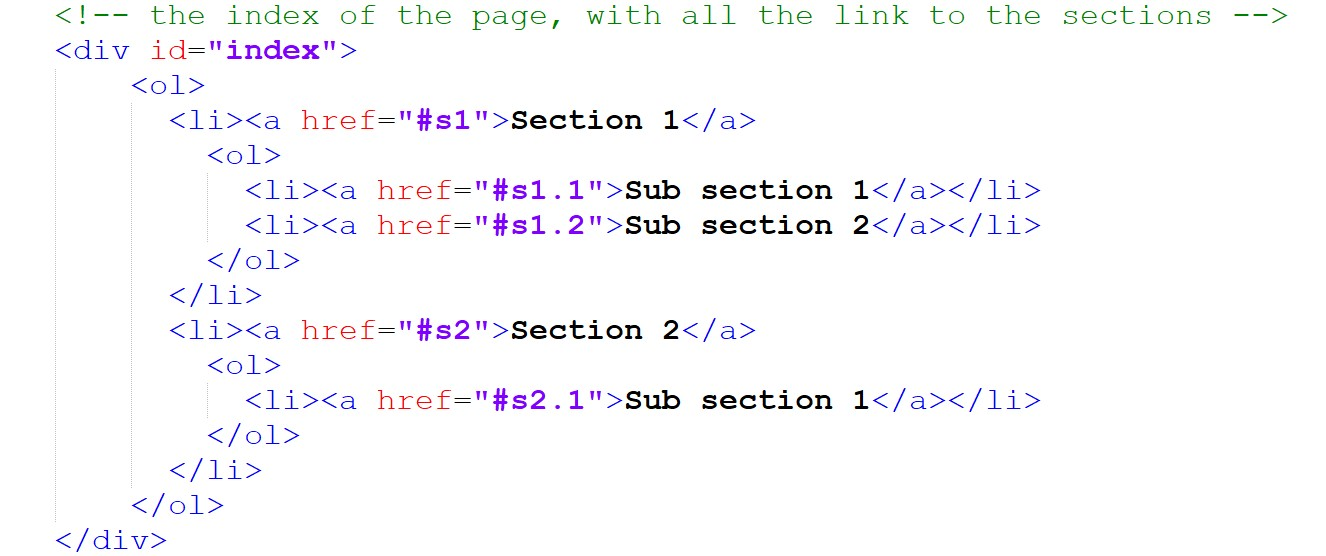
\includegraphics[height=6.4cm]{index.jpg}
    \end{figure}
    
    \item Check the validity of your page. Your page \textbf{must} pass the \colorbox{grey!7}{W3C validation}. \\
    \textit{Follow this link:} \texttt{\href{https://validator.w3.org/#validate_by_upload+with_options}{https://validator.w3.org/\#validate\_by\_upload+with\_options}}
    
    \item Once you have done all previous steps, add the folder to the repository using the command \colorbox{grey!7}{\texttt{svn add}}.\\
    \textit{Example:} \texttt{svn add web/html/gen0\_pong/}
    
    \item Lastly, you can commit your work using the command \colorbox{grey!7}{\texttt{svn commit}} with a message. \\
    \textit{Note: make sure to put an appropriate and reasonable message} \\
    \textit{Example:} \texttt{svn commit -m "added the page for pong gen0" web/html/gen0\_pong/}
    
\end{itemize}

\end{document}
